\chapter{Interpretation of Results}
\label{chap:Interpretation}

\indent Since no significant excesses where observed in the signal region, the results are interpreted as exclusions on stop parameter space.  The 95 percent confidence expected and observed exclusion limit is shown in figure \ref{figure.exclusion.SRC}.  The exclusion CL$_s$ are derived using the exclusion fit procedure described in section \ref{sec:stat:limit} where all 5 bins in $\RISR$ are simultaneously fitted and statistically combined. Previous 8 TeV stop exclusion limits are shown in blue for comparison. \\

\begin{figure}[htbp]
	\begin{center}
		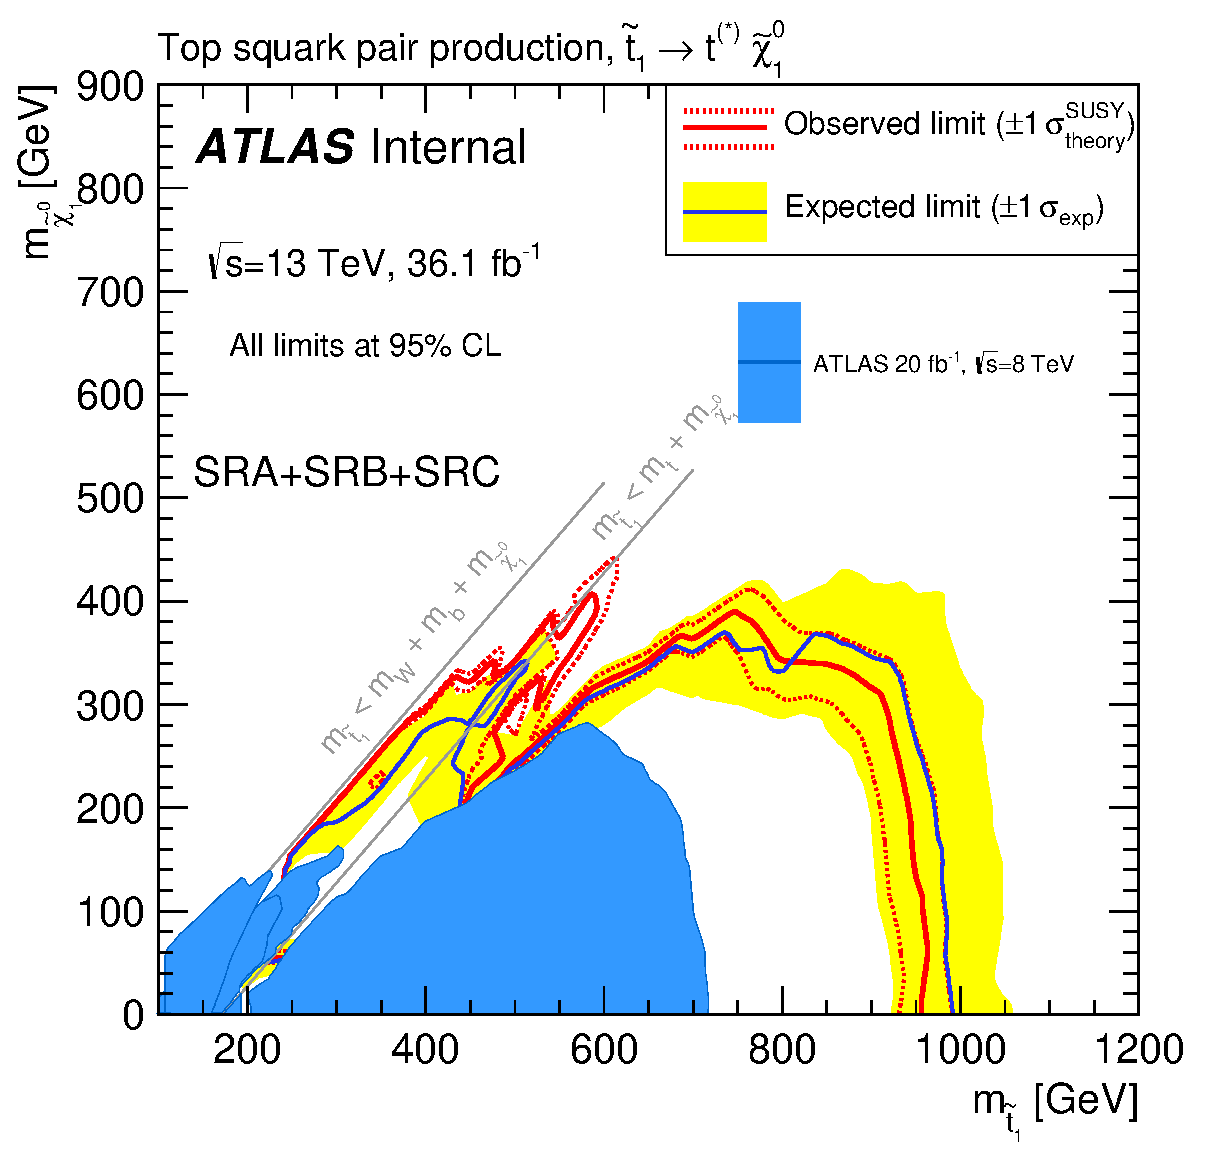
\includegraphics[width=0.85\textwidth]{figures/fit/atlascls_m0m12_wband1_showcms0_StopZL2016_SRABC_Tt_directTTplusbWN_all_Output_fixSigXSecNominal_hypotest__1_harvest_list.eps}
		\caption{Results of the exclusion fits in the tN1 grid from a simultaneous fit to the compressed analysis SR}
		\label{figure.exclusion.SRC}
	\end{center}
\end{figure}

\indent  The compressed stop analysis fills in the 8 TeV gap in exclusion along the $\Delta m = m_{t}$ diagonal line.  The analysis is able to exclude stops from $225 \gev$ to $600 \gev$ in this region with a CL$_s$ below $5\times 10^{-4}$ for stop mass between 250 and 400 $\gev$.  The analysis also extends the zero lepton sensitivity far into the 3 body decay region almost to the $\Delta m = m_{W}+m_{b}$ line. \\

\indent Figure \ref{figure.exclusion.SRABC} shows the compressed stop analysis exclusion limit (SRC) combined with the bulk region 13 TeV stop 0 lepton analysis exclusion limit (SRA+SRB).  The bulk stop 0 lepton analysis targets the high stop masses parameter space with large mass splitting between stop and neutralino masses.  The stop decay gives a large amount of momenta to the resulting neutralinos in regions with large mass splittings.  The bulk region analysis targets this kinematic feature and use large amount of $\met$ to separate signal from background.   Because of this, the bulk region analysis's strategy loses sensitivity as the $\Delta m$ approaches $m_{t}$.  A detail description of the bulk region stop 0 lepton analysis can be found in \cite{stop0Lmoriond}.  \\

\begin{figure}[htbp]
	\begin{center}
		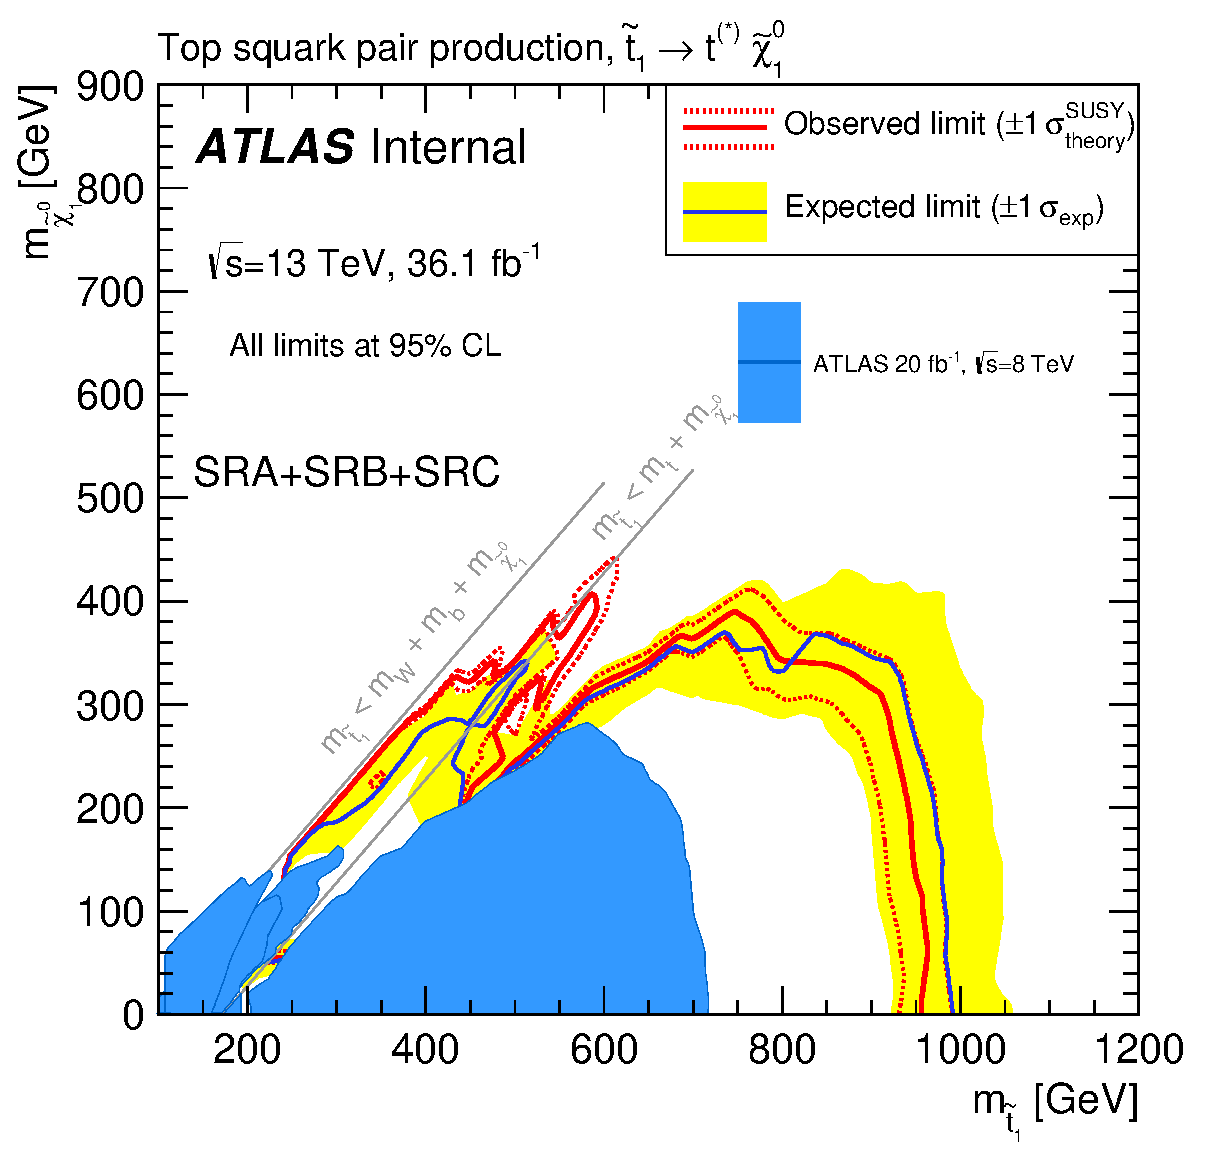
\includegraphics[width=0.85\textwidth]{figures/fit/atlascls_m0m12_wband1_showcms0_StopZL2016_SRABC_Tt_directTTplusbWN_all_Output_fixSigXSecNominal_hypotest__1_harvest_list.eps}
		\caption{Results of the exclusion fits in the tN1 grid from the combination of the bulk region stop 0L analysis (SRA+SRB) and the compressed analysis (SRC). The bulk region analysis SRA targets high stop masses with large $\Delta m$ and SRB targets high stop masses with medium amount of $\Delta m$.  SRC is the compressed region analysis and adds sensitivity to the $\Delta m = m_{t}$ diagonal region where SRA and SRB lack sensitivity. }
		\label{figure.exclusion.SRABC}
	\end{center}
\end{figure}

\indent Figure \ref{figure.exclusion.SRABCD_dm1} show how the exclusion limit on the stop/neutralino parameter space plane for different the branching fraction of $\stop \rightarrow t+\ninoone$ and $\stop \rightarrow b+\chinoonepm$.  As the $\stop \rightarrow t+\ninoone$ branching fraction decreases, the $\stop \rightarrow b+\chinoonepm$ branching fraction increases.  A new signal region {\tt SRD} that directly targets the mixed decay channel is added to the analysis.  Detailed documentation on the mixed decay analysis can also be found in \cite{stop0Lmoriond}.  Again the compressed analysis is responsible for the exclusion of all stop parameter space along the $\Delta m = m_{t}$ diagonal line when branching fraction to $\stop \rightarrow t+\ninoone$ is high. \\

\begin{figure}[htbp]
	\begin{center}
		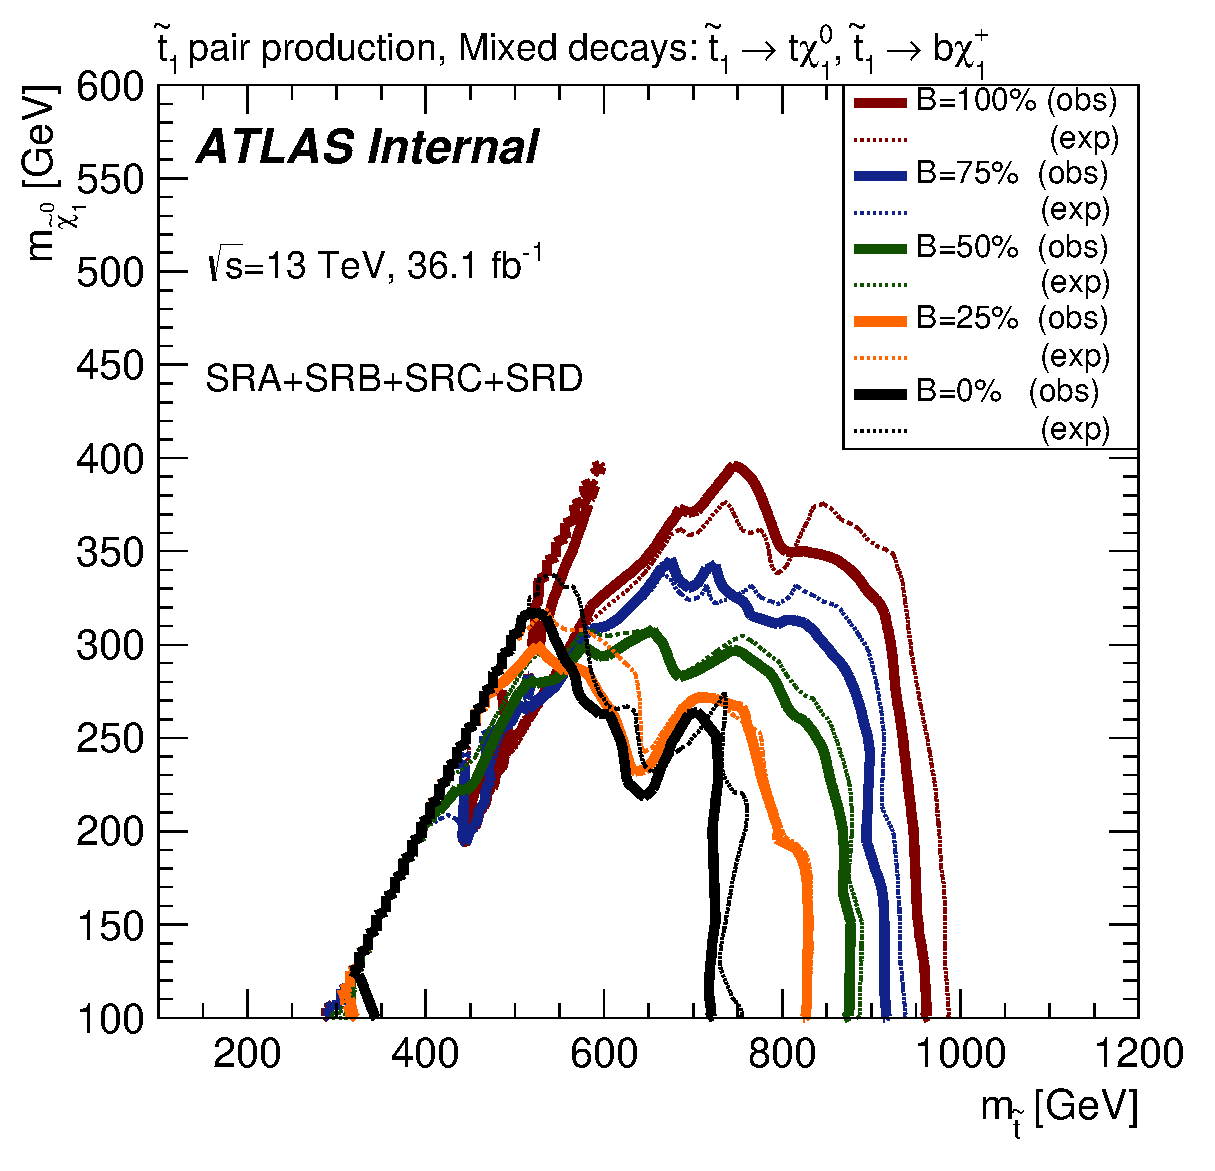
\includegraphics[width=0.85\textwidth]{figures/fit//SRABCD_mixed_dm1.eps}
		\caption{Results of the exclusion fits in the grid
                  with two stop decay channels: $\stop\ra t\ninoone$
                  and $\stop\ra b\chinoonepm\ra b
                  W^{(*)}\ninoone$, with $m(\chinoonepm)-m(\ninoone) =
                  1 GeV$.  The results are shown as a function of the
                  branching ratio to $\stop\ra t\ninoone$: 0\%, 25\%, 50\%, 75\% and 100\%.  
                  The results are based on taking the signal region with the best
                  expected $CL_s$, using SRA, SRB, SRC, and SRD.
                  SRA and SRB target high stop masses in the  $\stop\ra t\ninoone$ decay channel at high stop masses and moderate to large $\Delta m$.  SRC is the compressed region analysis that targets  $\stop\ra t\ninoone$ with $\Delta m \sim m_t$.  SRD targets a mix decay channel with branching fraction to both  $\stop\ra t\ninoone$ and $\stop\ra b\chinoonepm\ra b W^{(*)}\ninoone$.  We can see that the compressed analysis SRC adds sensitivity to the $\Delta m = m_t$ line when the branching fraction is mainly to $\stop\ra t\ninoone$.}
		\label{figure.exclusion.SRABCD_dm1}
	\end{center}
\end{figure}